\documentclass[9pt]{pnas-new}
% Use the lineno option to display guide line numbers if required.
% Note that the use of elements such as single-column equations
% may affect the guide line number alignment. 

%\RequirePackage[english,slovene]{babel} % when writing in slovene
\RequirePackage[slovene,english]{babel} % when writing in english

%\templatetype{pnasresearcharticle} % Choose template 
\templatetype{pnasresearcharticle} % = Template for a two-column research article
% {pnasmathematics} = Template for a one-column mathematics article
% {pnasinvited} = Template for a PNAS invited submission

\usepackage{subcaption}
\usepackage{graphicx}

%\selectlanguage{slovene}
%\etal{in sod.} % comment out when writing in english
%\renewcommand{\Authands}{ in } % comment out when writing in english
%\renewcommand{\Authand}{ in } % comment out when writing in english

\newcommand{\set}[1]{\ensuremath{\mathbf{#1}}}
\renewcommand{\vec}[1]{\ensuremath{\mathbf{#1}}}
\newcommand{\uvec}[1]{\ensuremath{\hat{\vec{#1}}}}
\newcommand{\const}[1]{{\ensuremath{\kappa_\mathrm{#1}}}} 

% Custom commands for Easier writing
\renewcommand{\etal}{et al.\ }
\newcommand{\eg}{e.g., }
\newcommand{\ie}{i.e., }
\newcommand{\wrt}{w.r.t. }
\newcommand{\etc}{etc.}
\newcommand{\na}{\emph{n.a.} }

\newcommand{\num}[1]{#1}

\title{Simulating Coral Competition and Growth under a Simulated Environment}

% Use letters for affiliations, numbers to show equal authorship (if applicable) and to indicate the corresponding author
\author{Nejc Hirci}

\affil{Collective behavior course research seminar report} 

% Please give the surname of the lead author for the running footer
\leadauthor{Hirci} 

\selectlanguage{english}

% Please add here a significance statement to explain the relevance of your work
\significancestatement{Significance Statements}{
Understanding coral competition and growth dynamics is vital for effective restoration in response to climate-induced threats to coral reefs. Inspired by Cresswell \etal~\cite{coral_community_3D}, we implement accretive growth principles in their proposed model, capturing diverse ecological processes.
}


% Please include corresponding author, author contribution and author declaration information
\authorcontributions{Please provide details of author contributions here.}
\authordeclaration{Please declare any conflict of interest here.}
\equalauthors{\textsuperscript{1}A.O.(Author One) and A.T. (Author Two) contributed equally to this work (remove if not applicable).}
\correspondingauthor{\textsuperscript{2}To whom correspondence should be addressed. E-mail: author.two\@email.com}

% Keywords are not mandatory, but authors are strongly encouraged to provide them. If provided, please include two to five keywords, separated by the pipe symbol, e.g:
\keywords{Coral simulation, collective behavior, procedural modeling} 

\begin{abstract}

This article introduces a new extension to coral simulation models, merging a three-dimensional cellular automata growth model with a complex model of coral growth. In response to climate-induced threats to coral reefs, understanding coral competition and growth dynamics is vital for effective restoration. Inspired by Cresswell \etal~\cite{coral_community_3D}, we implement accretive growth principles in their proposed model, capturing diverse ecological processes. Implemented with WebGPU compute shaders for parallelism, the model efficiently simulates multiple scales. Developed as a web application using Node.js and Typescript, the model integrates Babylon.js for realistic 3D rendering. This research contributes a visually compelling real-time simulation model, enhancing our understanding of coral community dynamics and offering insights crucial for reef restoration and conservation in the face of environmental challenges. While our implementation still requires much optimization, it is already publicly available on the following website 
\url{https://nejchirci.github.io/CoralSimulation}.
\end{abstract}

\dates{\textbf{\today}}
\program{BM-RI}
\vol{2023/24}
\no{CB:G1} % group ID
\fraca{FRIteza/201516.130}

\begin{document}

% Optional adjustment to line up main text (after abstract) of first page with line numbers, when using both lineno and twocolumn options.
% You should only change this length when you've finalised the article contents.
\verticaladjustment{-2pt}

\maketitle
\thispagestyle{firststyle}
\ifthenelse{\boolean{shortarticle}}{\ifthenelse{\boolean{singlecolumn}}{\abscontentformatted}{\abscontent}}{}

\section*{Introduction}

In marine biology, coral reefs have been an essential research subject for many years due to their importance in preserving marine wildlife and their naturally high biodiversity. Unfortunately, they are also one of the ecosystems most susceptible to the various environmental changes brought about by climate change. Much of current marine research focuses on the restoration efforts of coral reefs, for which it is crucial to understand the environmental factors that affect coral communities. For such purposes, we need ways to adequately simulate many complicated ecological processes in four dimensions. Much existing research focuses on empirically tested models, which provide essential simulation output variables (\eg coral communities coverage) but are often limited to two dimensions. While not directly concerned with full coral reef simulations, some recent studies showed impressive results~\cite{sponge_growth, inifinigen} in generating realistic three-dimensional coral models using different growth simulation approaches. Such models lack simulations of the middle and large-scale ecological processes (\eg bleaching and grazing) but can offer a good starting point for simulating individual coral growth. We propose extending an existing three-dimensional~\cite{coral_community_3D} coral reef model with a more complex growth model. Due to the complexity of computation needed to simulate such environments on multiple scales, we implement our solution relying on parallelism offered by WebGPU compute shaders. 

\section*{Related Work}

Most simulation models that focus on analyzing the behavior of coral reefs limit themselves to a two-dimensional setting because introducing another spatial dimension requires a considerably more complex growth model. They are still helpful in analyzing important secondary variables such as the percentage cover of each coral community, the number of new coral recruits, and the rugosity created by coral colonies. They form a theoretical baseline for some of the more recent three-dimensional models~\cite{coral_community_3D}.

One of the recent review studies by Weijerman \etal~\cite{coral_models_review} describes a precise categorization of ecological model design approaches based on their leading principles. One of the major leading principles is to design models suited for extrapolation and long-term projections of coral community dynamics. These models require complex sub-models of various ecological processes and often rely on prior research to achieve realistic long-term predictions. These approaches often accept a trade-off between system understanding and its predictive capabilities by using simpler sub-modules in their simulation. Compared to simpler data-driven models, they lose some of the robustness and interpretability of results but can provide long-term projections that are still useful in many practical scenarios.

Researchers often rely on individual or agent-based models to explore coral competition under changing conditions. They are well suited to introduce coral-community dynamics based on diversity, functional individual traits, and demography of a coral reef. Importantly, they can be used with submodels of varying complexity. This is seen in a recently developed model by Carturan \etal~\cite{coral_community_main}, extended with trait-based approaches from existing trait databases. Their model shows an extensive set of simulated ecological processes (bleaching, reproduction, sedimentation, algae invasion, \etc) and includes a set of 798 functionally realistic species defined using 11 functional traits carefully designed from empirical data. Given their model's complexity, it can be argued that a simple two-dimensional grid of cell agents is adequate to achieve suitable predictions of coral population dynamics. In our approach, we decided to simplify some processes to introduce a more complex three-dimensional coral growth model, albeit still based on cellular automata.

One of the more common criticisms against agent-based models is their complex analysis and validation, but well-defined design protocols have addressed this in recent years~\cite{agent_based_validation}. The proposed Overview, Design Concepts, and Details (ODD) protocol defines how to describe individual- and agent-based models. We follow their principles in describing our model.

Turning our attention to three-dimensional simulation models, one of the recent papers by Cresswell \etal~\cite{coral_community_3D} describes a three-dimensional functional-structural model, Coralcraft, focused on investigating the influence of hydrodynamic disturbances on coral communities. They simulate five different coral morphologies: encrusting, hemispherical, tabular, corymbose, and branching, with a three-dimensional cell grid. Light, shading, nutrient distribution, and hydrodynamic disturbances all influence the growth of each polyp. They cover major ecological processes, growth, recruitment, and mortality but lack some minor ones, like algae invasions, bleaching, and dislodgement. Nevertheless, they provide a reliable baseline we use in our work.

Most coral simulation models focus on providing useful projected variables that describe the health and state of a coral reef. They do not, however, in most cases concern themselves with providing geometrically realistic results. The reason is that modeling realistic coral growth is a complex problem, which may lower the robustness of a complex coral reef model.

While there have been only a few three-dimensional coral community dynamics models, we can find several three-dimensional growth models that provide somewhat realistic results. Most general models usually consider themselves modeling stone or soft corals. They have significant anatomical differences because stone corals form hard external calcium carbonate skeletons, while soft corals are held together by jelly-like mesoglea and internal rigid structures~\cite{corals_book_1983}. Due to this, most general coral growth models simulate one or the other. 

One of the well-established models presented by Merks \etal~\cite{polyp_growth} was one of the first to address growth on a polyp-level scale. Their growth schema starts from initial conditions, then performs voxelization to polyps, resource transport in the environment, and the accretion step of actual growth. Kaandorp \etal~\cite{Kaandorp_2013} later extended their work by introducing a fluid flow model and an extended model of the dispersion of nutrients by advection-diffusion. They also showed that their model can adequately simulate branching sponges and stone corals. Recent work by O'Hagan \etal~\cite{sponge_growth} noted that their accretive growth model may only partially fit to simulate the coral growth of sponges. They introduce an extension by improving the initial skeletal architecture and using an accretive growth model afterward.

In computer graphics, some research focuses more on creating realistic procedural models of corals without simulating the actual growth. A recent paper by Raistrick \etal ~\cite{inifinigen} proposed a comprehensive procedural generator that can produce numerous 3D scenes of the natural world. While it simulates many common natural phenomena such as fire, clouds, rain, \etc, it focuses only on providing an excellent visual presentation of the natural biomes. They describe many exciting approaches to procedurally model coral morphologies (leather corals, table corals, branching corals, \etc). While visually striking, these do not apply to simulation models with realistic growth projections.

In our work, we propose an extension to existing models~\cite{coral_community_3D} by providing useful visualizations of coral community dynamics but with a combination of a complex growth model based on accretive growth. We will implement our approach in a compute shader using the modern web graphics pipeline, WebGPU, and deploy a publicly available application.

\section*{Methods}

This section describes our CPU-based implementation of the three-dimensional cellular automata growth model mimicking the approach proposed in \textit{Coralcraft} and a proposed model validation.

As described in work by Cresswell \etal., the \textit{CoralCraft} model focuses on simulating the influence of hydrodynamic disturbances on coral communities. Their approach divides the model environment into $1cm^3$ voxels, representing the lowest spatial level at which all computation occurs, and are equivalent to one coral colony polyp.

The initial implementation captures the main ecological processes of growth, reproduction, mortality, and hydrodynamic disturbance. The model describes five possible functional morphologies, which represent a branching, tabular, encrusting, hemispherical, and corymbose coral, and can be seen in Figure~\ref{fig:morphologies}. The simulation step is equivalent to a week passed and proceeds in the following steps:


\begin{enumerate}
    \item Light attenuation and shading from existing coral colonies are computed at every voxel.
    \item Resources are distributed to coral polyps according to light levels.
    \item Coral polyps, with insufficient resources, die, which can lead to the colony's death.
    \item All live polyps are grown according to their colony morphologies.
\end{enumerate}

\begin{figure}[!htb]
    \centering
    \begin{subfigure}{0.3\textwidth}
        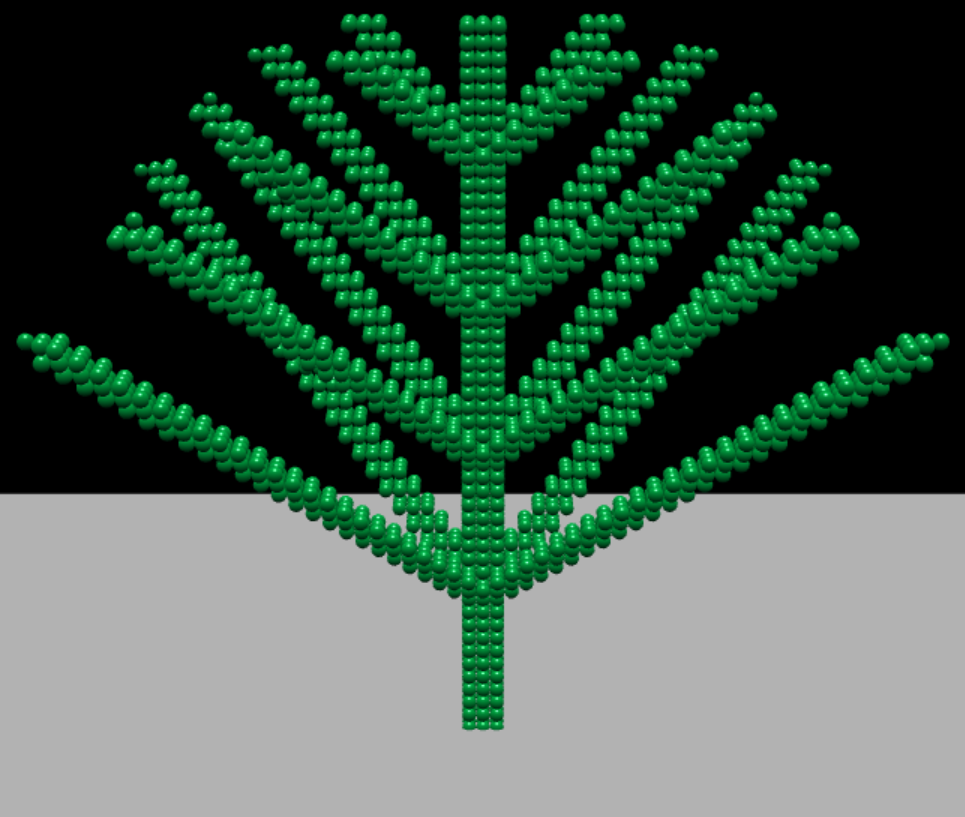
\includegraphics[width=\textwidth]{fig/branching.png}
        \caption{}
    \end{subfigure}
    \begin{subfigure}{0.3\textwidth}
        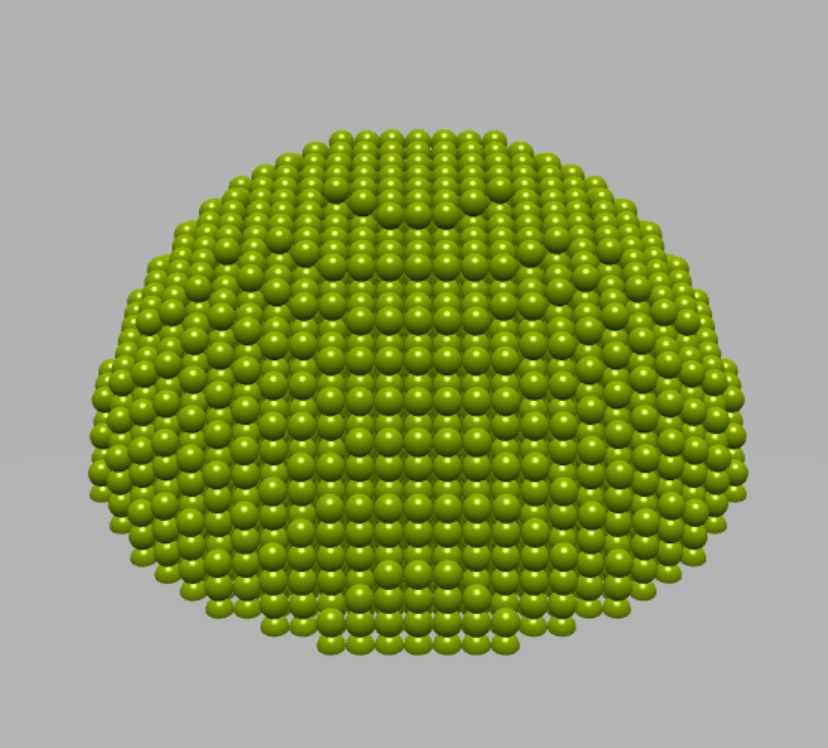
\includegraphics[width=\textwidth]{fig/hemispherical.png}
        \caption{}
    \end{subfigure}
    \begin{subfigure}{0.3\textwidth}
        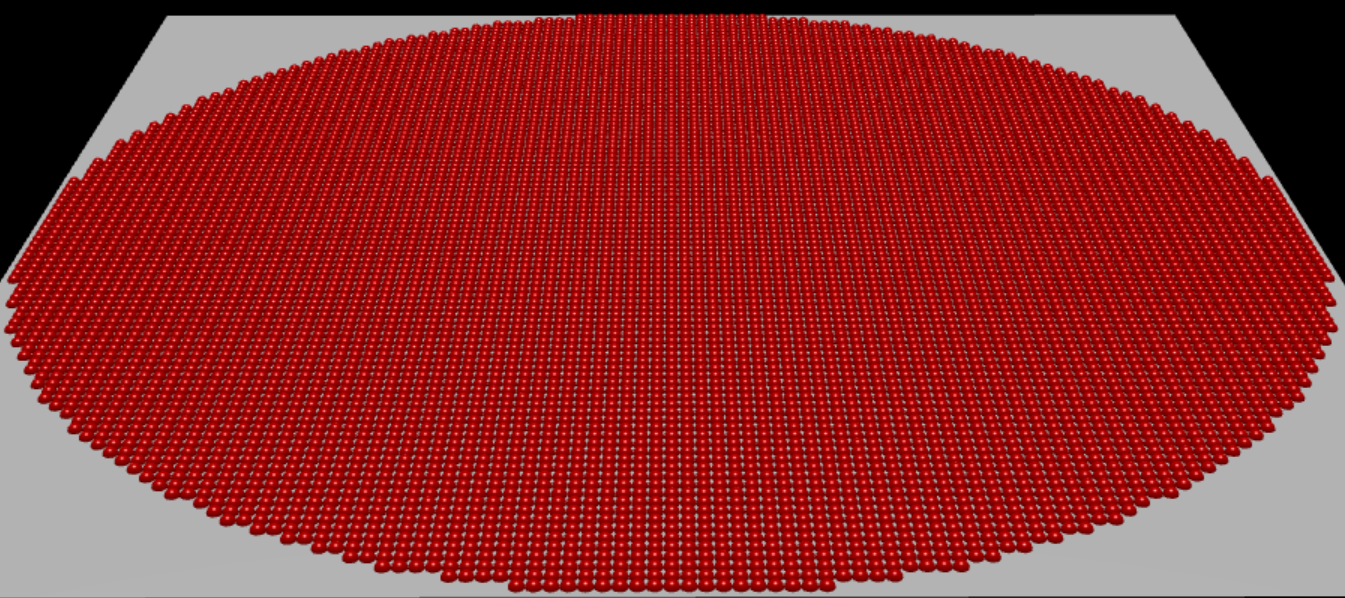
\includegraphics[width=\textwidth]{fig/encrusting.png}
        \caption{}
    \end{subfigure}
    \begin{subfigure}{0.3\textwidth}
        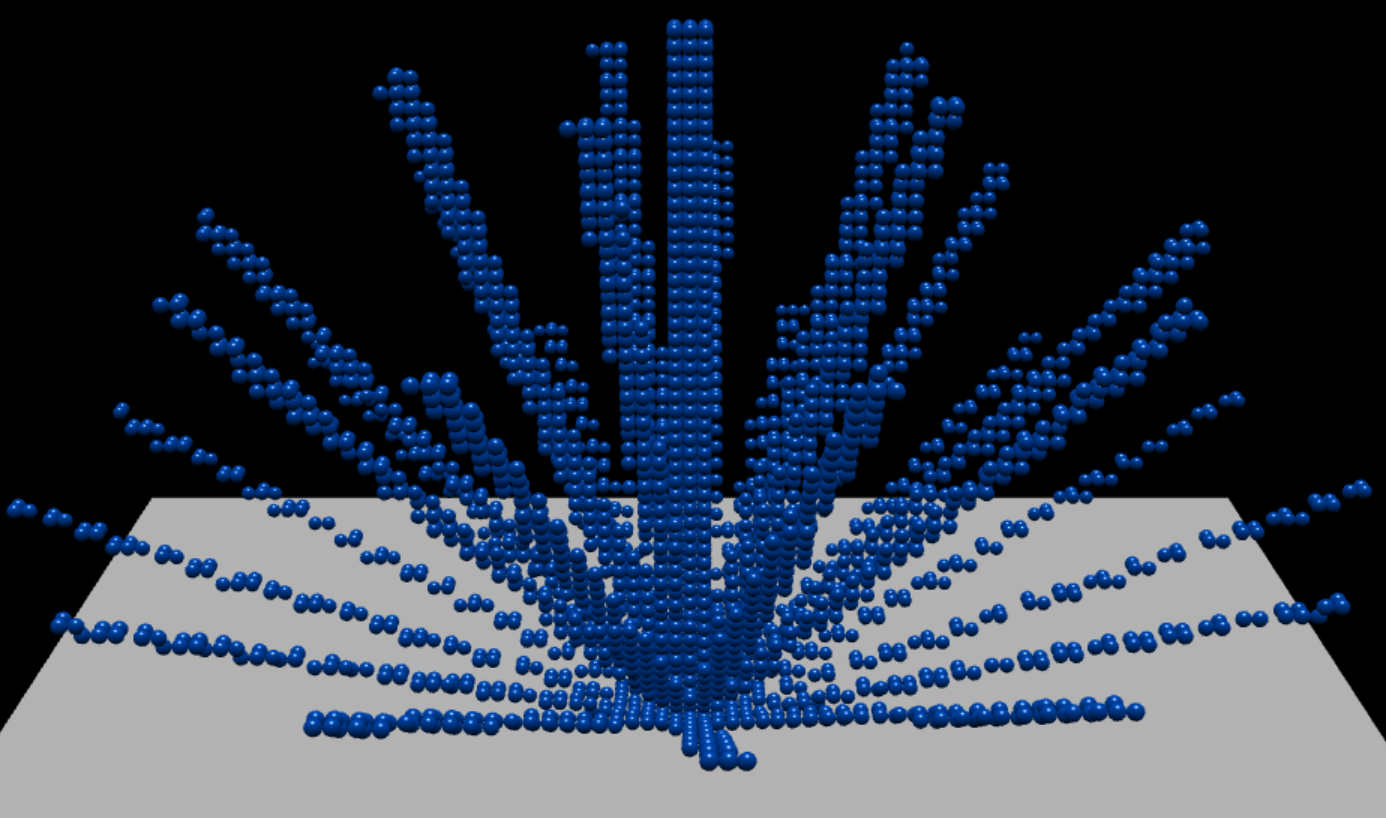
\includegraphics[width=\textwidth]{fig/corymbose.png}
        \caption{}
    \end{subfigure}
    \begin{subfigure}{0.3\textwidth}
        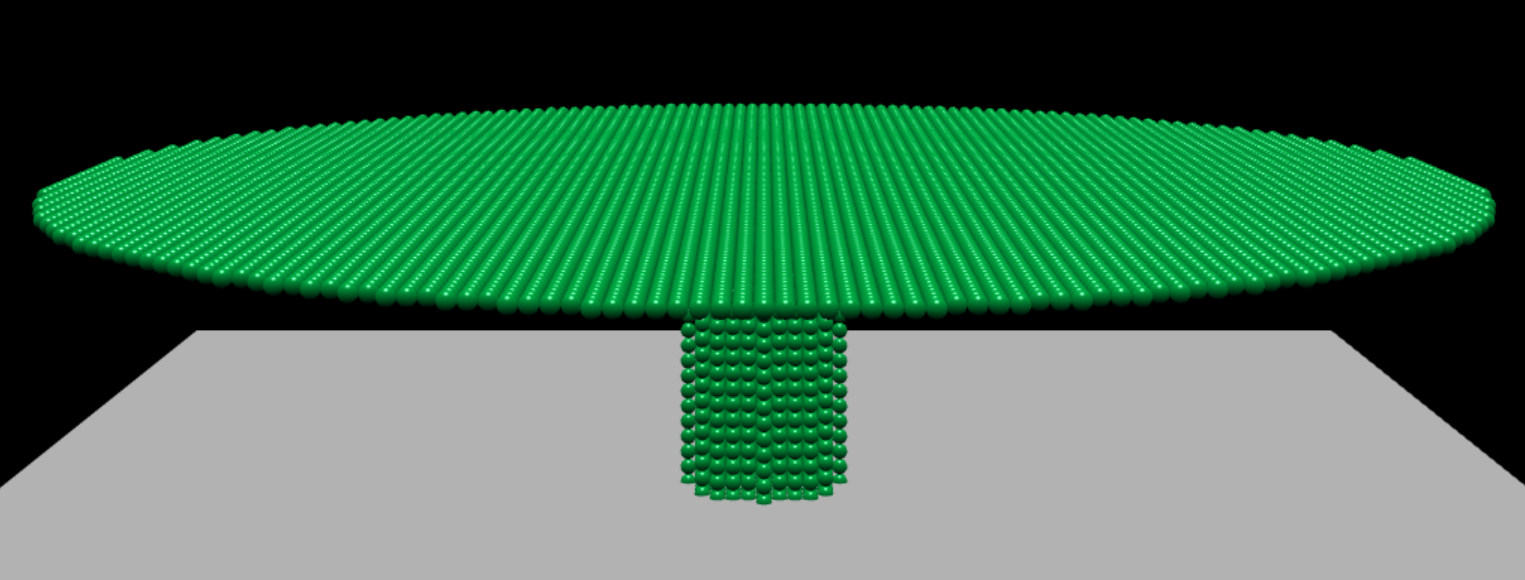
\includegraphics[width=\textwidth]{fig/tabular.png}
        \caption{}
    \end{subfigure}
    \caption{Five coral morphologies: (a) Branching, (b) Hemispherical, (c) Encrusting, (d) Corymbose, (e) Tabular.}
    \label{fig:morphologies}
\end{figure}

In addition, the reproduction and hydrodynamic disturbances are at different frequencies. Reproduction is simulated as a random occupation of voxels on the seafloor (y==0) once every year, where we choose the morphologies of recruits according to the number of all coral cells belonging to each of the five morphologies.

Notably, the initially proposed model integrated the impact of hydrodynamic disturbances by computing the colony shape factor (CSF). It is a dimensionless index of mechanical vulnerability to horizontal forces. The formula considers the side profile of the colony along with the size of the basal attachment to the sea floor. When a hydrodynamic disturbance occurs, we compute the CSF of each colony, which we use as the probability of the colony getting dislodged, which causes the death of the polyp cells.

We aimed to implement the first CPU-based version of the model, but we plan to validate its correctness in our following report. We will do that by tracking important output variables of the models as described in the original paper and comparing them to empirical data of a naturally growing coral reef. These variables are \textit{coral colony morphology density}, \textit{linear rugosity}, which describes the level of branching of the whole reef, \textit{morphological diversity}, and the \textit{occupied volume of each morphology}. 

We develop a web application with the simulation model using established web development technologies, such as Node.js~\cite{nodejs} and the Typescript programming language. We use a publicly available library Babylon.js~\cite{babylonjs} for rendering the 3D scene. For the next version of the implementation, we plan to add more realistic rendering and a faster simulation computation using WebGPU~\cite{webgpu} compute shaders.

%. With that, we will be able to establish that our fluid and nutrient simulations work correctly and assess their model's performance. Next, we plan to introduce an accretive growth coral model as initially presented by Merks \etal. We will consider how we can closely model three of the morphologies shown in Coralcraft. We will focus more on the functional representation of the coral models because simulating realistic growth will be out of our work's scope. As a last inclusion, we will extend our model with additional ecological processes critical to coral reef dynamics, like bleaching and dislodgement, which will, in turn, influence our growth model. We plan to validate our model by observing simulation outputs, like percentage cover, volume, and colony density, and comparing them to existing case studies of specific coral reefs.

%We will implement a web-based application of our model, relying on established web development technologies, such as Node.js~\cite{nodejs} and Typescript programming language, to provide a publicly available website with our proposed model. Our initial model implementation will rely only on a CPU-based simulation algorithm. Still, due to the complexity of coral growth, we anticipate that a GPU-based implementation will be needed. The new web graphical API, WebGPU~\cite{webgpu}, offers support for using compute shaders for performing various computations in parallel on the GPU. We plan to leverage the robust capabilities it provides to implement the calculation of our simulation. Because rendering underwater environments is a complex problem that requires the implementation of many specific light phenomena (\eg caustics), we provide only a simple rendering of our simulation using an established rendering library Three.js~\cite{threejs}.

\section*{Results}

Our implemented model shows promising results in the simulation of the coral growths. We have yet to validate the produced output with empirical real-world data, but we can already see many parameters working as expected.

\begin{figure}[!htb]
    \centering
    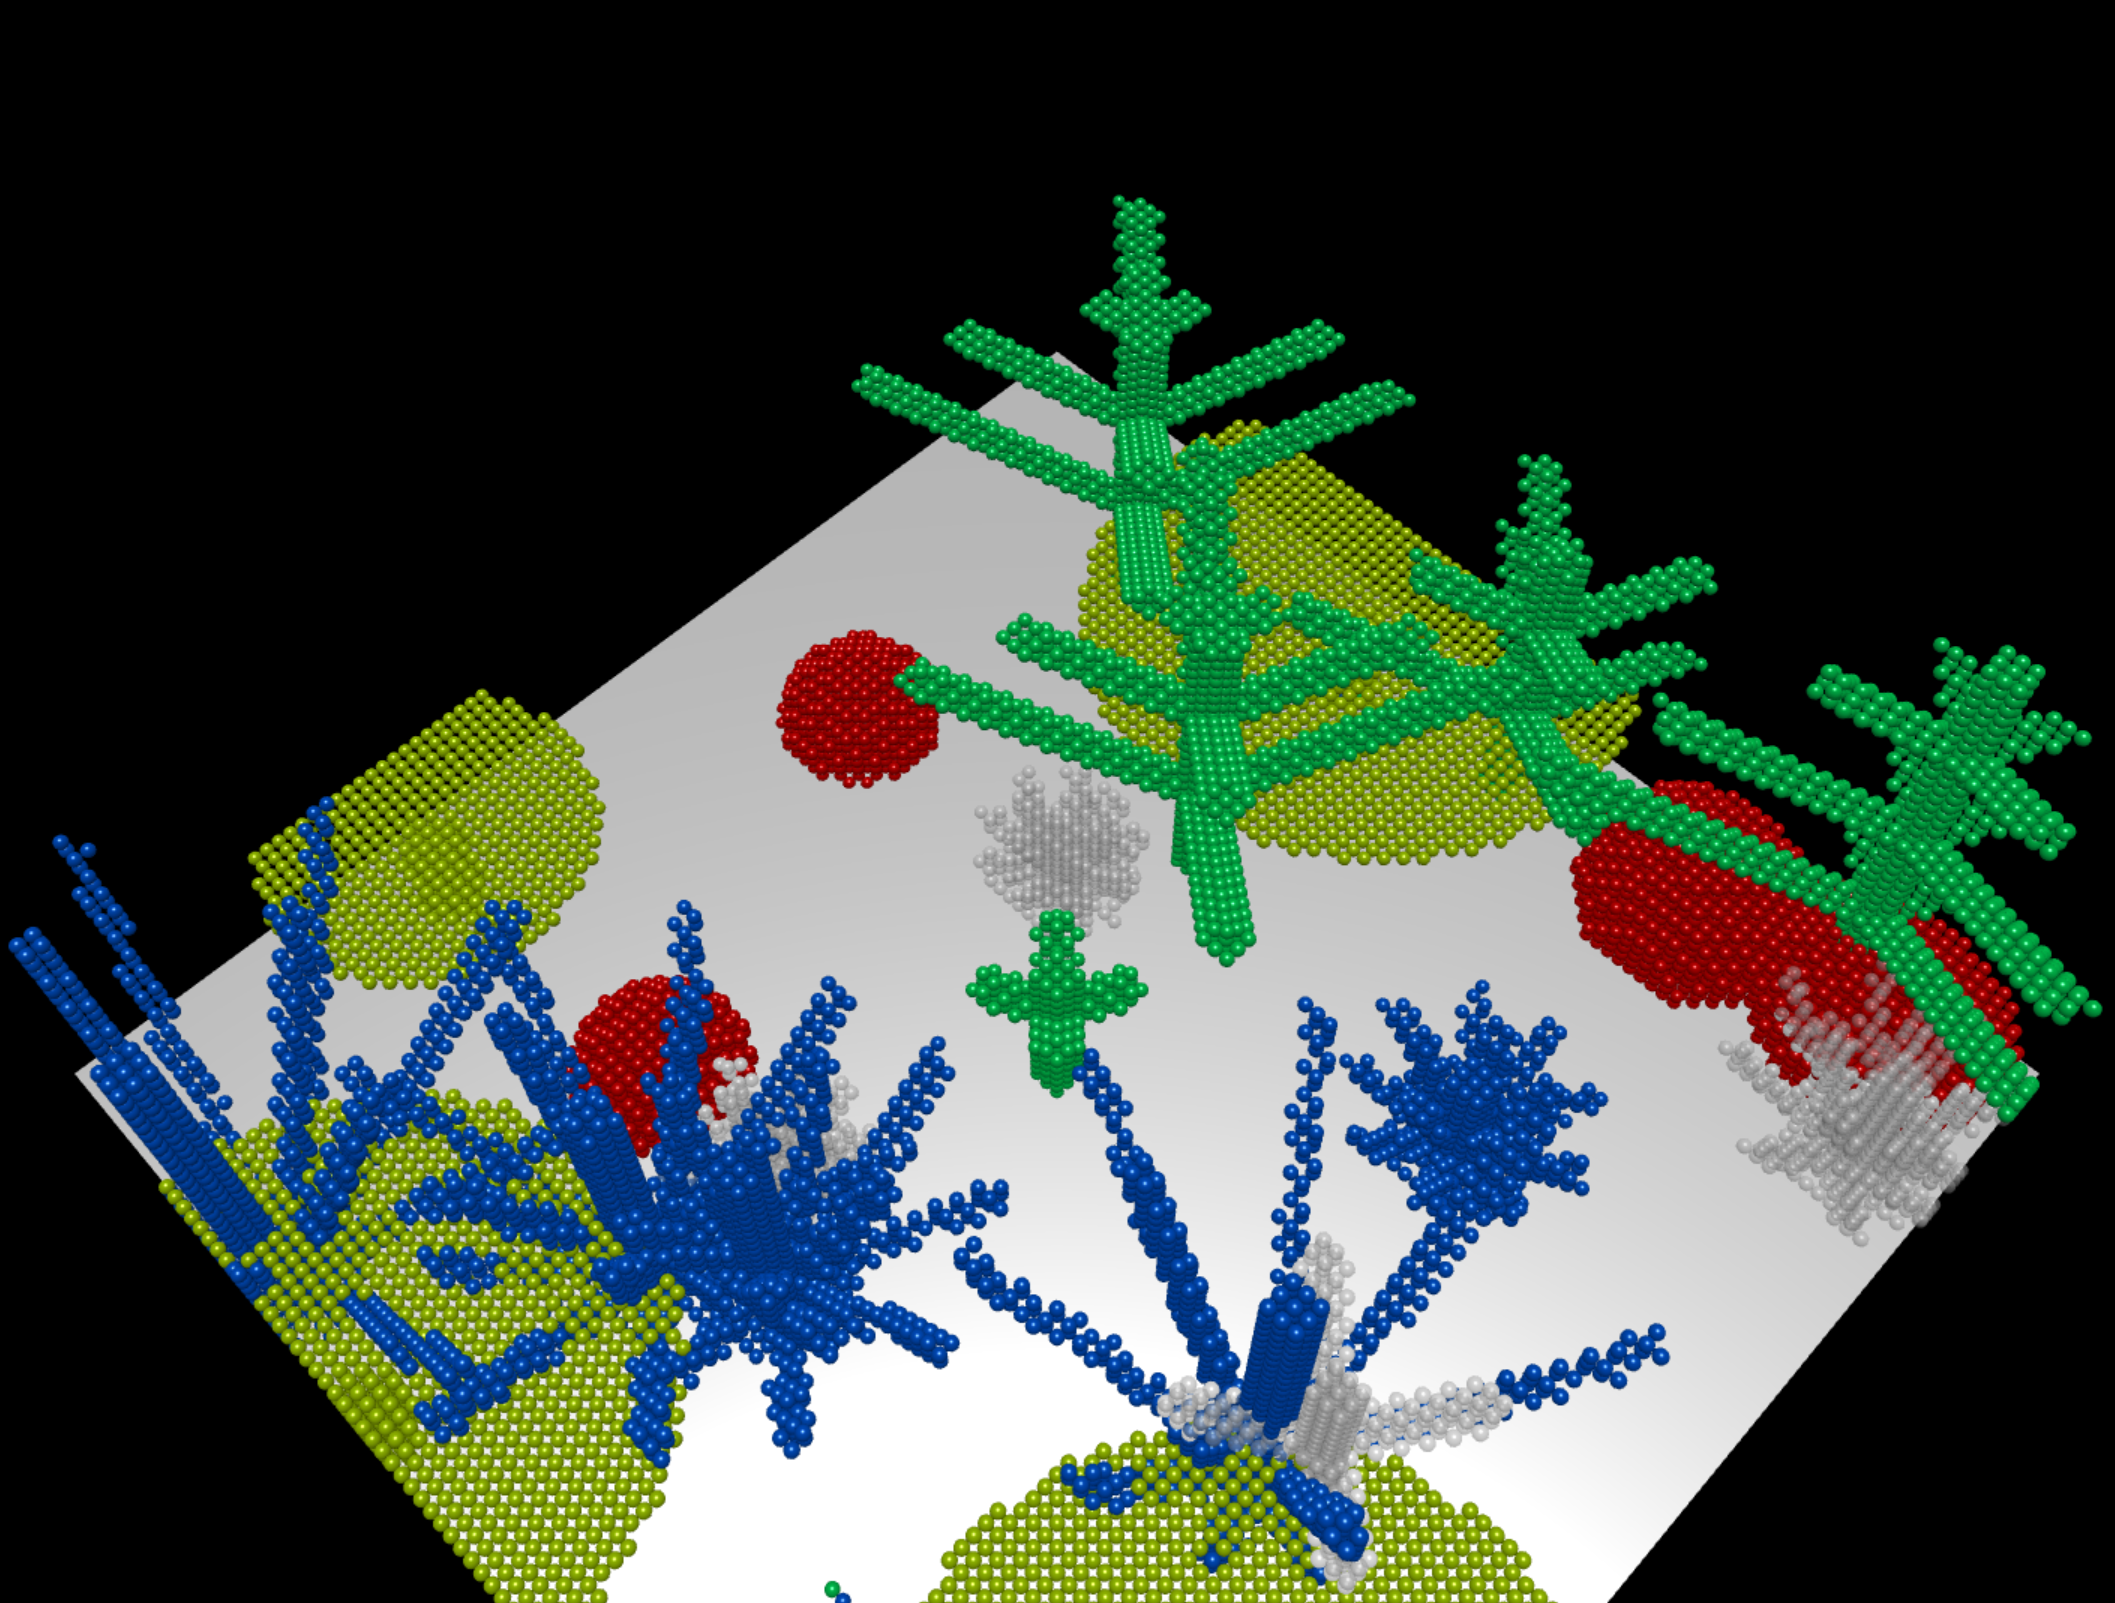
\includegraphics[width=0.7\textwidth]{fig/simulation_2.png}
    \caption{Example of initial implementation.}
    \label{fig:simulation}
\end{figure}

In Figure~\ref{fig:simulation}, we can see an example of a simulation after a couple of years. The current visual representation uses a very simplistic rendering model, where all polyps are rendered as colored spheres. Each colony is colored appropriately depending on its morphology class, with the grayed-out cells representing dead colonies. 

\section*{Discussion}

Observing initial results, we can already see the expected higher death rate of branching and corymbose corals. Their death is mainly due to their faster growth at the expense of coral skeleton stability, which leads to a lower coral shape factor.

We want to comment that the current model implementation is a recreation of the original paper and, as such, lacks the proper optimization required for real-time use and interaction. We will rewrite the implementation to be executed with GPU-based compute shaders to achieve that, considerably increasing the performance. After that, we will improve the growth model and validate its results. The validation will utilize the empirical data offered in the original paper based on the extracted simulation variables described in the previous section. Lastly, we will extend the user interface with control of the simulation parameters and visualization of validation metrics described in the previous section. 

\section*{Conclusion}

While we are happy with our ability to reproduce the proposed coral simulation model successfully, the current implementation still requires much optimization. As previously stated, we also want to improve the current coral growth model to mimic the visual appearance of real-life corals more closely.

% \pnasbreak splits and balances the columns before the references.
% If you see unexpected formatting errors, try commenting out this line
% as it can run into problems with floats and footnotes on the final page.
%\pnasbreak

\begin{multicols}{2}
\section*{\bibname}
% Bibliography
\bibliography{./bib/bibliography}
\end{multicols}

\end{document}